\documentclass[border=6pt]{standalone}
\usepackage{pgfplots}
\pgfplotsset{compat=1.18}
\usepgfplotslibrary{groupplots}
\definecolor{cbblue}{HTML}{4C9BD1}
\begin{document}
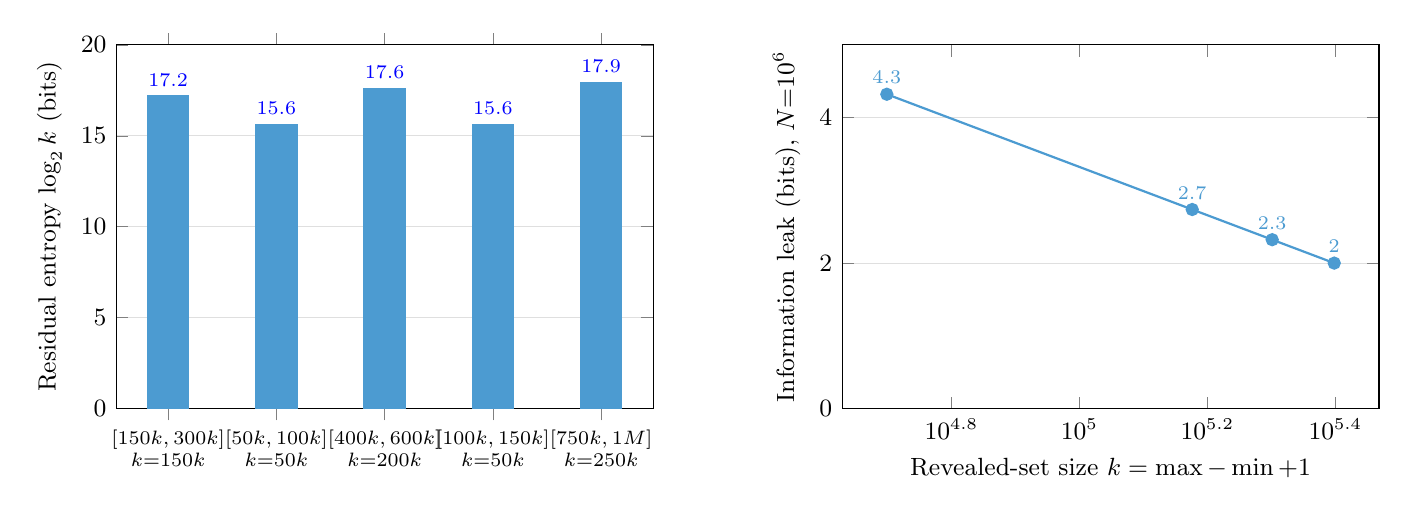
\begin{tikzpicture}
\begin{groupplot}[
  group style={group size=2 by 1, horizontal sep=2.4cm},
  width=8.4cm, height=6.2cm,
  tick label style={font=\small}, label style={font=\small},
  ymajorgrids, grid style={gray!25},
]
% ---- (a) residual entropy per predicate ----
\nextgroupplot[
  ybar, bar width=15pt,
  ymin=0, ymax=20,
  ylabel={Residual entropy $\log_2 k$ (bits)},
  symbolic x coords={deed1,deed2,deed3,deed4,deed5},
  xtick=data,
  xticklabels={%
    {$[150k,300k]$\\$k{=}150k$},%
    {$[50k,100k]$\\$k{=}50k$},%
    {$[400k,600k]$\\$k{=}200k$},%
    {$[100k,150k]$\\$k{=}50k$},%
    {$[750k,1M]$\\$k{=}250k$}},
  xticklabel style={align=center, font=\scriptsize},
  enlarge x limits=0.12,
  nodes near coords={\pgfmathprintnumber[precision=1]{\pgfplotspointmeta}},
  every node near coord/.append style={font=\scriptsize},
]
\addplot+[fill=cbblue, draw=cbblue] coordinates
  {(deed1,17.195)(deed2,15.610)(deed3,17.610)(deed4,15.610)(deed5,17.932)};

% ---- (b) information leak vs interval width ----
\nextgroupplot[
  xmode=log,
  xlabel={Revealed-set size $k=\max-\min+1$},
  ylabel={Information leak (bits), $N{=}10^{6}$},
  ymin=0, ymax=5,
  nodes near coords={\pgfmathprintnumber[precision=1]{\pgfplotspointmeta}},
  every node near coord/.append style={font=\scriptsize, anchor=south},
]
\addplot+[mark=*, cbblue, thick, mark options={fill=cbblue}] coordinates
  {(50001,4.322)(150001,2.737)(200001,2.322)(250001,2.000)};
\end{groupplot}
\end{tikzpicture}
\end{document}
